\chapter{Qiskit}\label{ch:qiskit}
This chapter describes a solution that we use for programming quantum computers and working with quantum algorithms. 

Do not confuse programming a quantum computer with standard high-level programming as we know it from classical computers, we are not there yet. The programming of quantum computers is more like programming in assembly language. In assembly language, you have to be aware of the hardware and the architecture of the computer, and using some low-level instructions we manipulate the hardware. The same principle is applied here, we have qubits and we manipulate them using quantum gates. For this purpose, we decided to go with an open-source Qiskit (Quantum Information Science Kit) library for Python backed by IBM.

There are also other alternatives like Cirq (by Google), Pennylane (by Xanadu), Q\# (by Microsoft), Sliq (by ETH Zürich), and many more. \ques{should I include citations to these libraries/companies?} The reason why we decided on Qiskit is that it serves our purpose and it is far ahead of its competitors and competitors offer nowhere near what Qiskit offers. It is the most popular quantum computing library, it provides a lot of learning resources, tutorials, videos, and as it is open source there is a big community around it. IBM has built an entire ecosystem around it \cite{qiskit_ecosystem} with libraries for quantum machine learning, chemistry, finance, and many more. The 7-year work of IBM culminated in the middle of February 2024, when they released version 1.0.0. of Qiskit. Even though Qiskit is mainly developed by IBM, it is not limited to IBM's quantum computers, through additional packages can support a hardware of other companies.

\subsection{Quantum simulator}
\todo{explain how we can simulate quantum computers on a classical computer}\\
\\
\todo{VQE is probably a better place for paragraphs below}
Before we dive into benchmarking our ansatzes we need to make clear a few terms.

\begin{definition} (Shots) 
    A shot is a single run of a quantum circuit. As we know from the previous chapters, the quantum computation is probabilistic. The results of individual shots can be different. The more shots we run, the more accurate the results are.
\end{definition}

In the below picture, we can see a distribution of measurements when using different numbers of shots. Each one of the states is equally likely. With an increasing number of shots, we can observe that the distribution converges to a uniform distribution.

\begin{figure}[H]
    \centering
    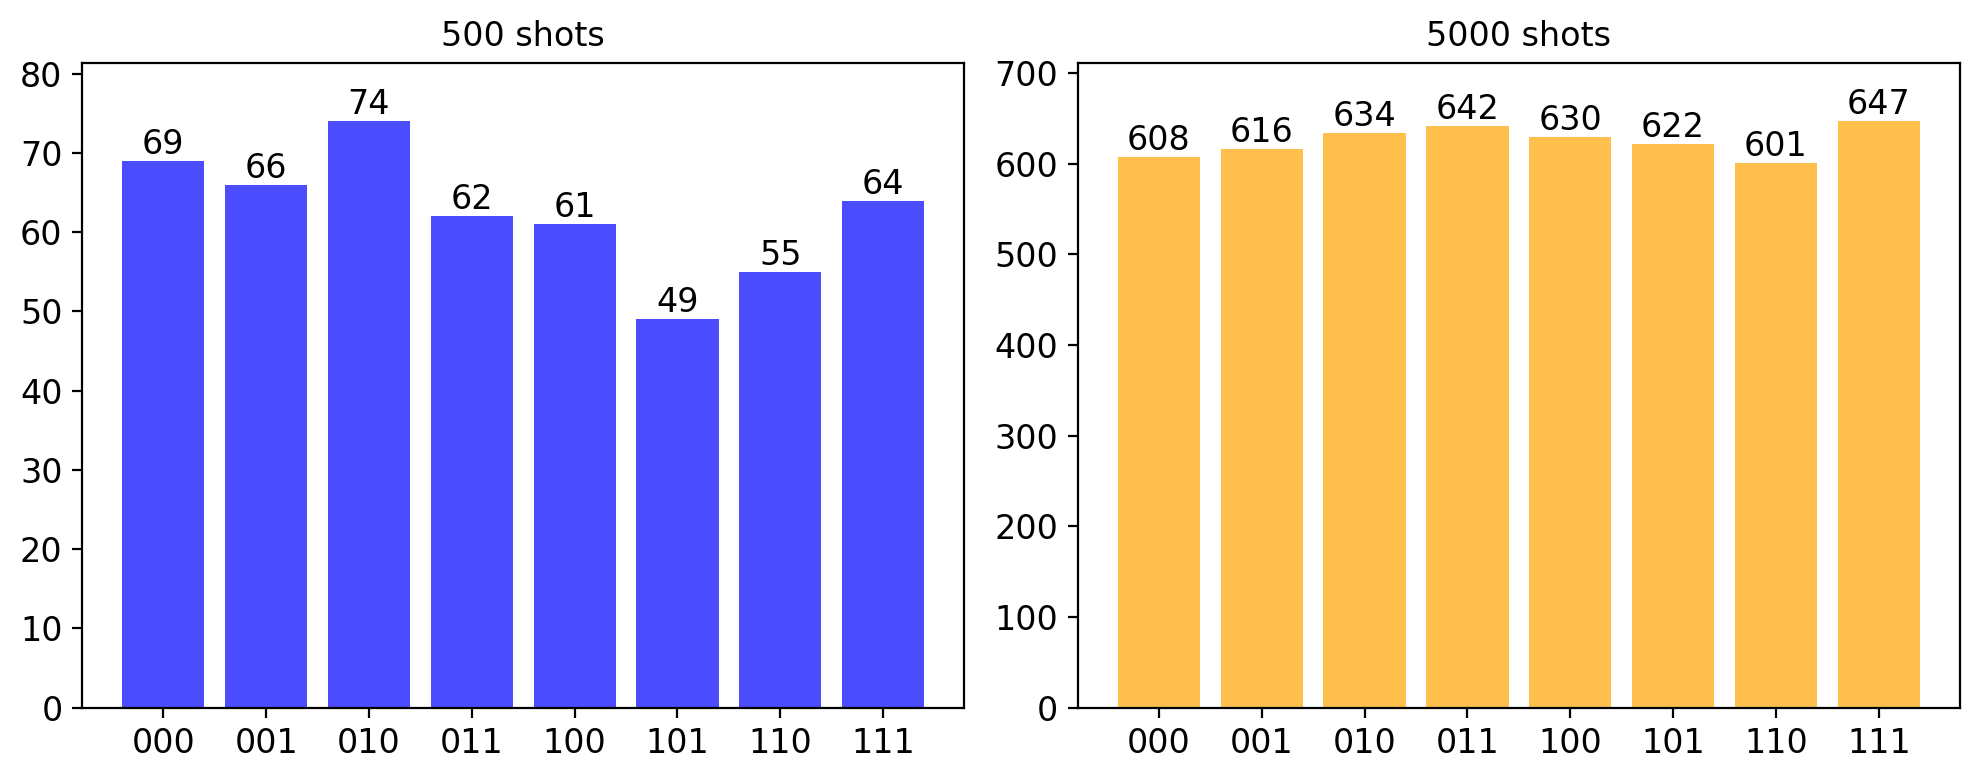
\includegraphics[width=\linewidth]{shots-distribution.png}
    \caption{Measurement distribution for different numbers of shots.}\label{fig:output}
\end{figure}

\begin{definition} (Iteration) 
    An iteration is a single run of the VQE, thus run a quantum circuit to find an expectation value of the Hamiltonian and then use the classical optimizer to find the best parameters for the next iteration.
\end{definition}

\begin{definition}(Function evaluation)
    Our cost function is passed to a classical optimizer which tries to determine the best parameters that can lead to minimal value. Function evaluations are a number of how many times the cost function was evaluated. Therefore in a single iteration can optimizer evaluate the cost function multiple times.
\end{definition}

\todo{HarTree}\\
\todo{Initial point}\\
\todo{Hyperparameters}\\
\todo{("fault-tolerant QPUs") FTQC vs NISQ}\\
\todo{UCC vs HEA https://arxiv.org/pdf/2310.02511.pdf}\\
\todo{Divide shots into stages}\\
\todo{commutative hamiltonian}\\
